\documentclass[10pt]{article}
\usepackage{icmlko}

\icmlmeta{IP 파운데이션 월드모델}{157}{판이 쓰는 축과 팝업이 쓰는 축이 다르다}{노트 156이 ``한 칸 올려도 순위가 3\%밖에 안 움직인다''를 남겼다. 손 축 다섯과 외부 축 열넷을 갈라 보니, 판을 만드는 것과 팝업을 만드는 것이 서로 다른 무더기였다}

\begin{document}

\twocolumn[
\icmlheader

\begin{abstract}
노트 156의 마지막 줄이 ``축 한 칸을 올려도 순위가 3\%밖에 안 움직인다 ---
외부 축이 열아홉 중 열넷인데 그 비율부터 재라''였다. 갈랐다. 손 축 다섯
(타깃 폭 · 장소 노출 · 입장 마찰 · 미디어 푸시 · 굿즈 규모)과 외부 축 열넷
(검색 넷 · 달력 여섯 · 위키 넷)을 각각만 남기고 재 봤다. \textbf{두 무더기가
서로 다른 것을 만들고 있었다.} F18 배깅 기준으로, 판 $\rho$ 는 전부 쓸 때
$+$0.4495이고 손 축만 쓰면 $+$0.3525로 내려간다 --- \textbf{판의 $+$0.097은
외부 축이 만든다.} 그런데 팝업은 정반대다. 전부 쓰면 $+$0.4698인데
\textbf{손 축만 쓰면 $+$0.5026이고, 외부 축만 쓰면 $+$0.0874다.} 능형에서는
더 벌어진다 --- 손 축만 $+$0.5435, 외부 축만 $+$0.1785. \textbf{팝업의
예측력은 거의 전부 손 축 다섯에서 나온다.} 이유는 자료 성질이다: 판은 표본
수 가중이라 웹툰 27\% · 애니 23\% · 모바일 17\%가 지배하고 그 셋은 검색 ·
위키 덮음이 높은데, 팝업은 위키 덮음이 0\%이고 달력은 전 도메인 공통이라
변별이 없다. \textbf{다만 팝업 쪽 차이는 안 갈린다} --- 손 축만이 전부보다
$+$0.0446 $\pm$ 0.0653($t{=}0.7$), F18 에서 $+$0.0328 $\pm$
0.0706($t{=}0.5$)이다. $n{=}59$의 벽이 또 나온다. 갈리는 것은 하나뿐이고
그것은 크다 --- \textbf{외부 축만으로는 팝업을 못 맞힌다}($-$0.38). 마지막으로
노트 156의 물음에 답했다. 외부 축을 빼면 개입 효과 크기가 0.0341에서
0.0455로 \textbf{33\% 는다} --- 희석이 맞다. 그런데 \textbf{사전 부호 일치는
81\%에서 72\%로 떨어진다}(능형은 78\%$\to$58\%). \textbf{외부 축은 통제
변수 노릇을 하고 있었다} --- 크기를 깎는 대신 부호를 지킨다.
\end{abstract}
]

\begin{figure*}[t]
\centering
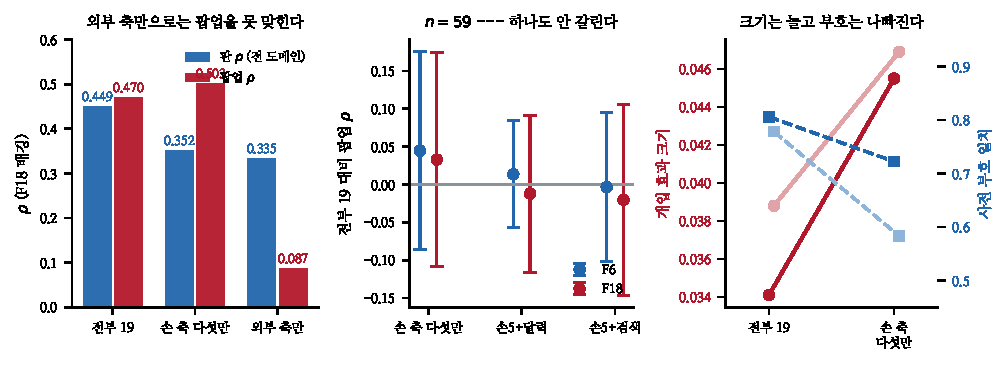
\includegraphics[width=\textwidth]{figs/split.pdf}
\caption{왼쪽 --- 외부 축만으로는 팝업을 못 맞힌다. 가운데 --- 팝업 쪽
차이는 하나도 안 갈린다. 오른쪽 --- 외부 축을 빼면 크기는 늘고 부호는
나빠진다.}
\end{figure*}

\section{두 무더기가 서로 다른 것을 만든다}

\begin{table}[t]
\centering\tsize
\caption{축 세트를 갈라서. 마스크로 비우고 잰다.}
\begin{tabular}{lrrrr}
\toprule
& \multicolumn{2}{c}{F18 배깅} & \multicolumn{2}{c}{F6 능형} \\
& 판 & 팝업 & 판 & 팝업 \\
\midrule
전부 19 & \textbf{$+$.4495} & $+$.4698 & \textbf{$+$.3667} & $+$.4989 \\
손 축 다섯만 & $+$.3525 & \textbf{$+$.5026} & $+$.3413 & \textbf{$+$.5435} \\
외부 축만 & $+$.3345 & \textbf{$+$.0874} & $+$.2382 & \textbf{$+$.1785} \\
\bottomrule
\end{tabular}
\end{table}

\claimx{\textbf{판의 $+$0.097은 외부 축이 만들고, 팝업의 거의 전부는 손 축이
만든다.} 외부 축 열넷만 주면 팝업이 $+$0.087(F18) · $+$0.179(F6)로
주저앉는다 --- 열넷을 다 줘도 손 축 다섯의 6분의 1이다.}{자료 성질로
설명된다. 판은 표본 수 가중이라 웹툰 · 애니 · 모바일이 67\%이고 그 셋은
검색 · 위키 덮음이 높다. 팝업은 위키가 0\%이고 달력은 전 도메인 공통이라
변별이 안 된다. 남는 것이 검색뿐인데 그것도 $+$0.09 어치다.}

\section{그런데 팝업 쪽은 안 갈린다}

\begin{table}[t]
\centering\tsize
\caption{팝업 $\rho$. 전부 19 대비. 재추출 400.}
\begin{tabular}{lrr}
\toprule
& F6 능형 & F18 배깅 \\
\midrule
손 축 다섯만 & $+$.0446 $\pm$ .0653 & $+$.0328 $\pm$ .0706 \\
손5$+$달력 & $+$.0135 $\pm$ .0352 & $-$.0121 $\pm$ .0518 \\
손5$+$검색 & $-$.0034 $\pm$ .0491 & $-$.0202 $\pm$ .0629 \\
\bottomrule
\end{tabular}
\end{table}

\claimx{\textbf{하나도 안 갈린다} --- $t$ 가 $-$0.3에서 $+$0.7이다. ``팝업에는
손 축만 쓰는 게 낫다''는 읽기가 눈에 보이지만 잴 수가 없다.}{노트 148이
이미 세운 벽이다. $n{=}59$ 에서 짝 반폭이 0.12이고 여기 차이들은 0.05
아래다. \textbf{점수를 보고 축 세트를 고르면 노트 139가 잡은 그
잘못이다} --- 안쪽 창으로 도메인별 축을 고르면 여섯 중 셋에서 순위가 음의
상관이었다.}

\claimx{\textbf{갈리는 것은 하나뿐이고 그것은 크다.} 외부 축만 쓰면 팝업이
$-$0.38 내려간다. 이건 어떤 오차막대로도 안 덮인다.}{그래서 이 노트가
확정하는 것은 ``손 축이 낫다''가 아니라 \textbf{``외부 축만으로는 팝업이
안 된다''}이다.}

\section{노트 156의 물음 --- 왜 3\%인가}

\begin{table}[t]
\centering\tsize
\caption{외부 축을 빼면.}
\begin{tabular}{lrrl}
\toprule
& 효과 크기 & 사전 부호 & \\
\midrule
F18 · 전부 19 & .0341 & \textbf{81\%} & \\
F18 · 손 축만 & \textbf{.0455} & 72\% & 크기 $+$33\% \\
\midrule
F6 · 전부 19 & .0388 & \textbf{78\%} & \\
F6 · 손 축만 & \textbf{.0469} & 58\% & 크기 $+$21\% \\
\bottomrule
\end{tabular}
\end{table}

\claimx{\textbf{희석이 맞다 --- 그러나 값을 치르고 산 것이다.} 외부 축을
빼면 개입 효과가 33\% 커지는데 사전 부호 일치가 9\%p 떨어진다. 능형에서는
20\%p나 떨어져 58\%로 동전에 가까워진다.}{\textbf{외부 축은 통제 변수
노릇을 하고 있었다.} 검색량 · 계절 · 위키 관심도를 빼면 손 축이 그
교란을 대신 빨아들이고, 그러면 계수가 커지는 대신 방향이 틀린다.}

\claimx{\textbf{그래서 ``3\%밖에 안 움직인다''는 결함이 아니다.} 통제를
제대로 걸었을 때의 크기가 그만큼이다. 통제를 빼서 4.5\%로 키울 수는
있지만 그 4.5\%는 방향이 덜 믿을 만하다.}{그렇다고 3\%가 충분하다는 뜻은
아니다. 기획자가 굿즈를 한 등급 키워 순위가 3\% 오른다면, 그것이 의사결정을
바꿀 만한 크기인지는 별개 문제다.}

\begin{table}[t]
\centering\tsize
\caption{남은 것.}
\begin{tabular}{ll}
\toprule
판정치 & 판과 팝업이 다른 축을 쓴다 --- 한 순위표로 둘 다? \\
통제 & 외부 축이 통제라면 더 넣으면 부호가 더 좋아지나 \\
크기 & 3\%가 의사결정을 바꾸는 크기인가 \\
\bottomrule
\end{tabular}
\end{table}

둘째 줄이 곧바로 잴 수 있는 것이다. 외부 축을 열넷에서 더 늘리면 --- 예컨대
노트 149의 위키 축을 팝업에도 붙이면 --- 사전 부호 일치가 더 오를 것이라는
예측이 선다. \textbf{예측이 서면 그것이 다음 실험이다.}

\end{document}
